% Options for packages loaded elsewhere
\PassOptionsToPackage{unicode}{hyperref}
\PassOptionsToPackage{hyphens}{url}
%
\documentclass[
]{book}
\usepackage{amsmath,amssymb}
\usepackage{lmodern}
\usepackage{ifxetex,ifluatex}
\ifnum 0\ifxetex 1\fi\ifluatex 1\fi=0 % if pdftex
  \usepackage[T1]{fontenc}
  \usepackage[utf8]{inputenc}
  \usepackage{textcomp} % provide euro and other symbols
\else % if luatex or xetex
  \usepackage{unicode-math}
  \defaultfontfeatures{Scale=MatchLowercase}
  \defaultfontfeatures[\rmfamily]{Ligatures=TeX,Scale=1}
\fi
% Use upquote if available, for straight quotes in verbatim environments
\IfFileExists{upquote.sty}{\usepackage{upquote}}{}
\IfFileExists{microtype.sty}{% use microtype if available
  \usepackage[]{microtype}
  \UseMicrotypeSet[protrusion]{basicmath} % disable protrusion for tt fonts
}{}
\makeatletter
\@ifundefined{KOMAClassName}{% if non-KOMA class
  \IfFileExists{parskip.sty}{%
    \usepackage{parskip}
  }{% else
    \setlength{\parindent}{0pt}
    \setlength{\parskip}{6pt plus 2pt minus 1pt}}
}{% if KOMA class
  \KOMAoptions{parskip=half}}
\makeatother
\usepackage{xcolor}
\IfFileExists{xurl.sty}{\usepackage{xurl}}{} % add URL line breaks if available
\IfFileExists{bookmark.sty}{\usepackage{bookmark}}{\usepackage{hyperref}}
\hypersetup{
  pdftitle={Climate Labs Incubation Program},
  pdfauthor={Université de Lorraine, PUCPR},
  hidelinks,
  pdfcreator={LaTeX via pandoc}}
\urlstyle{same} % disable monospaced font for URLs
\usepackage{longtable,booktabs,array}
\usepackage{calc} % for calculating minipage widths
% Correct order of tables after \paragraph or \subparagraph
\usepackage{etoolbox}
\makeatletter
\patchcmd\longtable{\par}{\if@noskipsec\mbox{}\fi\par}{}{}
\makeatother
% Allow footnotes in longtable head/foot
\IfFileExists{footnotehyper.sty}{\usepackage{footnotehyper}}{\usepackage{footnote}}
\makesavenoteenv{longtable}
\usepackage{graphicx}
\makeatletter
\def\maxwidth{\ifdim\Gin@nat@width>\linewidth\linewidth\else\Gin@nat@width\fi}
\def\maxheight{\ifdim\Gin@nat@height>\textheight\textheight\else\Gin@nat@height\fi}
\makeatother
% Scale images if necessary, so that they will not overflow the page
% margins by default, and it is still possible to overwrite the defaults
% using explicit options in \includegraphics[width, height, ...]{}
\setkeys{Gin}{width=\maxwidth,height=\maxheight,keepaspectratio}
% Set default figure placement to htbp
\makeatletter
\def\fps@figure{htbp}
\makeatother
\setlength{\emergencystretch}{3em} % prevent overfull lines
\providecommand{\tightlist}{%
  \setlength{\itemsep}{0pt}\setlength{\parskip}{0pt}}
\setcounter{secnumdepth}{5}
\usepackage{booktabs}
\ifluatex
  \usepackage{selnolig}  % disable illegal ligatures
\fi
\usepackage[]{natbib}
\bibliographystyle{apalike}

\title{Climate Labs Incubation Program}
\author{Université de Lorraine\footnote{\url{https://erpi.univ-lorraine.fr/}}, PUCPR\footnote{\url{https://erpi.univ-lorraine.fr/}}}
\date{2021-03-17}

\begin{document}
\maketitle

{
\setcounter{tocdepth}{1}
\tableofcontents
}
\hypertarget{welcome-to-clip}{%
\chapter*{Welcome to CLIP}\label{welcome-to-clip}}
\addcontentsline{toc}{chapter}{Welcome to CLIP}

Remember each Rmd file contains one and only one chapter, and a chapter is defined by the first-level heading \texttt{\#}.

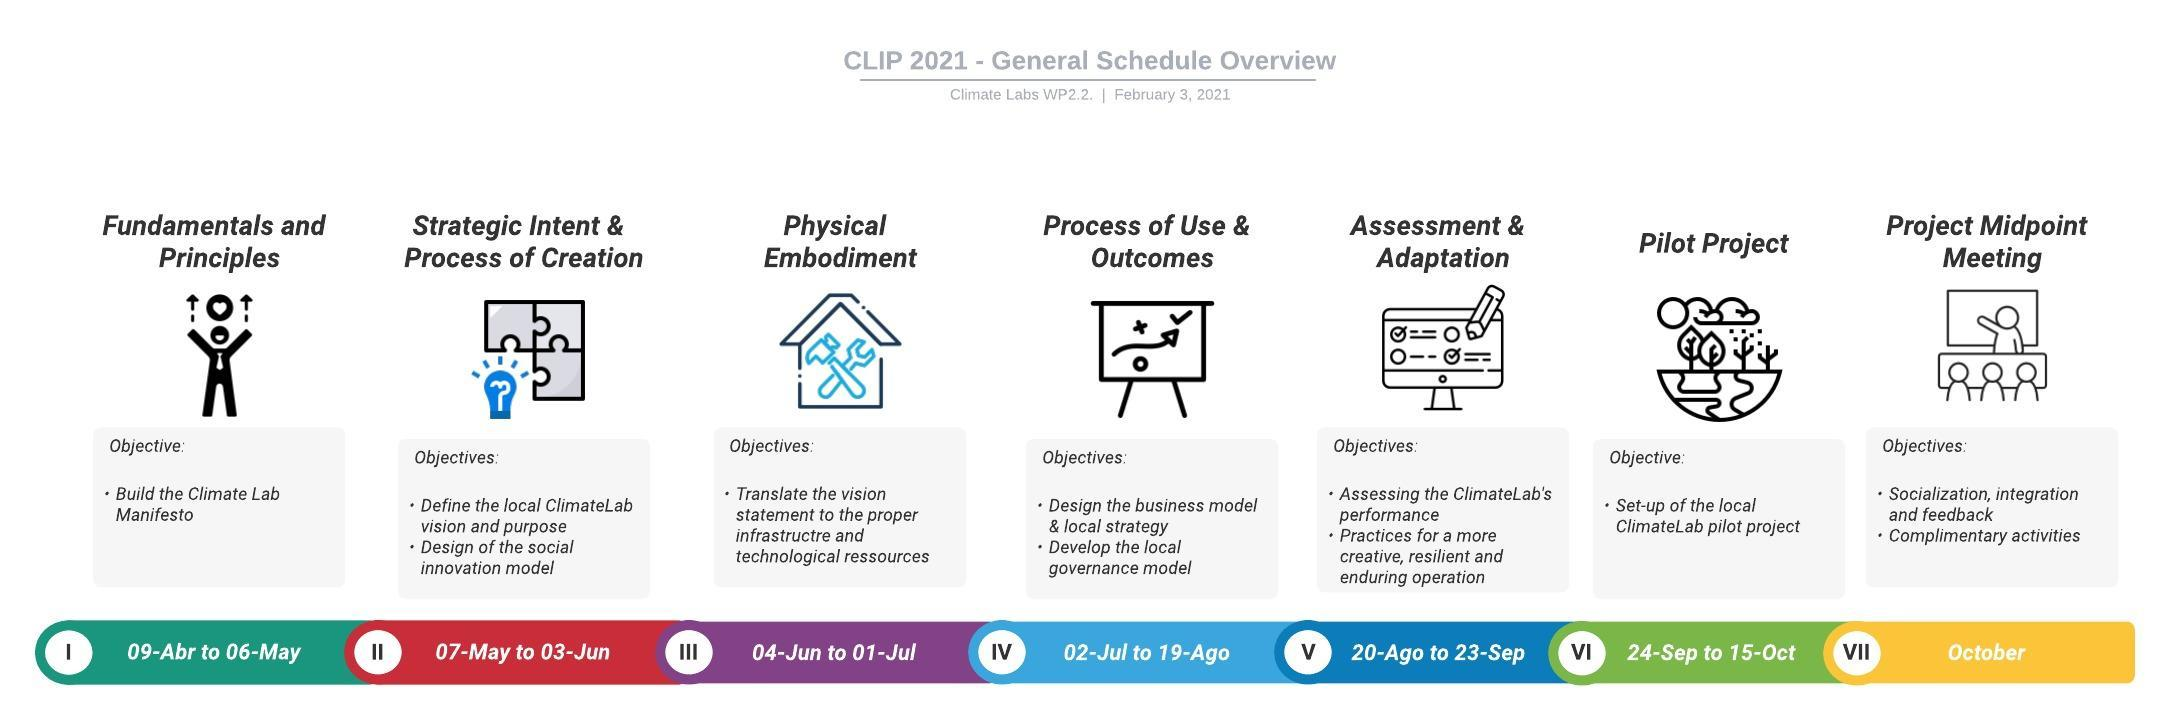
\includegraphics{Figures/CLIP-global-00.jpg}

\hypertarget{introduction}{%
\chapter*{Introduction}\label{introduction}}
\addcontentsline{toc}{chapter}{Introduction}

\hypertarget{purpose}{%
\chapter*{Purpose}\label{purpose}}
\addcontentsline{toc}{chapter}{Purpose}

This is the introduction to CLIP

\hypertarget{intro}{%
\chapter{Fundamentals and Principles}\label{intro}}

\hypertarget{intro-1}{%
\section{Intro}\label{intro-1}}

Welcome to the Fundamentals and prin

\begin{quote}
the main goal is \ldots{}
\end{quote}

\hypertarget{presentation}{%
\section{Presentation}\label{presentation}}

Here the presentation

\hypertarget{things-to-do}{%
\section{Things to do}\label{things-to-do}}

TAsk to do at the en with your CLT

\hypertarget{references}{%
\section{References}\label{references}}

Figures and tables with captions will be placed in \texttt{figure} and \texttt{table} environments, respectively.

Reference a figure by its code chunk label with the \texttt{fig:} prefix, e.g., see Figure \ref{fig:nice-fig}. Similarly, you can reference tables generated from \texttt{knitr::kable()}, e.g., see Table \ref{tab:nice-tab}.

\begin{table}

\caption{\label{tab:nice-tab}Here is a nice table!}
\centering
\begin{tabular}[t]{rrrrl}
\toprule
Sepal.Length & Sepal.Width & Petal.Length & Petal.Width & Species\\
\midrule
5.1 & 3.5 & 1.4 & 0.2 & setosa\\
4.9 & 3.0 & 1.4 & 0.2 & setosa\\
4.7 & 3.2 & 1.3 & 0.2 & setosa\\
4.6 & 3.1 & 1.5 & 0.2 & setosa\\
5.0 & 3.6 & 1.4 & 0.2 & setosa\\
\addlinespace
5.4 & 3.9 & 1.7 & 0.4 & setosa\\
4.6 & 3.4 & 1.4 & 0.3 & setosa\\
5.0 & 3.4 & 1.5 & 0.2 & setosa\\
4.4 & 2.9 & 1.4 & 0.2 & setosa\\
4.9 & 3.1 & 1.5 & 0.1 & setosa\\
\addlinespace
5.4 & 3.7 & 1.5 & 0.2 & setosa\\
4.8 & 3.4 & 1.6 & 0.2 & setosa\\
4.8 & 3.0 & 1.4 & 0.1 & setosa\\
4.3 & 3.0 & 1.1 & 0.1 & setosa\\
5.8 & 4.0 & 1.2 & 0.2 & setosa\\
\addlinespace
5.7 & 4.4 & 1.5 & 0.4 & setosa\\
5.4 & 3.9 & 1.3 & 0.4 & setosa\\
5.1 & 3.5 & 1.4 & 0.3 & setosa\\
5.7 & 3.8 & 1.7 & 0.3 & setosa\\
5.1 & 3.8 & 1.5 & 0.3 & setosa\\
\bottomrule
\end{tabular}
\end{table}

You can write citations, too. For example, we are using the \textbf{bookdown} package \citep{R-bookdown} in this sample book, which was built on top of R Markdown and \textbf{knitr} \citep{xie2015}.

\hypertarget{strategic-intend-process-of-creation}{%
\chapter{Strategic Intend \& Process of Creation}\label{strategic-intend-process-of-creation}}

\hypertarget{intro-2}{%
\section{Intro}\label{intro-2}}

Welcome to the Fundamentals and prin

\begin{quote}
the main goal is \ldots{}
\end{quote}

\hypertarget{things-to-do-at-the-end-of-this-sprint}{%
\section{Things to do at the end of this Sprint}\label{things-to-do-at-the-end-of-this-sprint}}

TAsk to do at the en with your CLT

\hypertarget{purpose-presentation-of-this-sprint}{%
\section{Purpose Presentation of this Sprint}\label{purpose-presentation-of-this-sprint}}

Here the presentation

\hypertarget{strategic-intent}{%
\subsection{Strategic Intent}\label{strategic-intent}}

\hypertarget{process-of-creation}{%
\subsection{Process of Creation}\label{process-of-creation}}

\hypertarget{references-1}{%
\section{References}\label{references-1}}

\hypertarget{physical-embodiment}{%
\chapter{Physical Embodiment}\label{physical-embodiment}}

\hypertarget{intro-3}{%
\section{Intro}\label{intro-3}}

Welcome to the Fundamentals and prin

\begin{quote}
the main goal is \ldots{}
\end{quote}

\hypertarget{things-to-do-at-the-end-of-this-sprint-1}{%
\section{Things to do at the end of this Sprint}\label{things-to-do-at-the-end-of-this-sprint-1}}

TAsk to do at the en with your CLT

\hypertarget{purpose-presentation-of-this-sprint-1}{%
\section{Purpose Presentation of this Sprint}\label{purpose-presentation-of-this-sprint-1}}

Here the presentation

\hypertarget{references-2}{%
\section{References}\label{references-2}}

\hypertarget{process-of-use-and-outputs}{%
\chapter{Process of Use and Outputs}\label{process-of-use-and-outputs}}

\hypertarget{intro-4}{%
\section{Intro}\label{intro-4}}

Welcome to the Fundamentals and prin

\begin{quote}
the main goal is \ldots{}
\end{quote}

\hypertarget{things-to-do-at-the-end-of-this-sprint-2}{%
\section{Things to do at the end of this Sprint}\label{things-to-do-at-the-end-of-this-sprint-2}}

TAsk to do at the en with your CLT

\hypertarget{purpose-presentation-of-this-sprint-2}{%
\section{Purpose Presentation of this Sprint}\label{purpose-presentation-of-this-sprint-2}}

Here the presentation

\hypertarget{references-3}{%
\section{References}\label{references-3}}

\hypertarget{assessment-adaptation}{%
\chapter{Assessment \& Adaptation}\label{assessment-adaptation}}

\hypertarget{intro-5}{%
\section{Intro}\label{intro-5}}

Welcome to the Fundamentals and prin

\begin{quote}
the main goal is \ldots{}
\end{quote}

\hypertarget{things-to-do-at-the-end-of-this-sprint-3}{%
\section{Things to do at the end of this Sprint}\label{things-to-do-at-the-end-of-this-sprint-3}}

TAsk to do at the en with your CLT

\hypertarget{purpose-presentation-of-this-sprint-3}{%
\section{Purpose Presentation of this Sprint}\label{purpose-presentation-of-this-sprint-3}}

Here the presentation

\hypertarget{references-4}{%
\section{References}\label{references-4}}

\hypertarget{pilot-project}{%
\chapter{Pilot Project}\label{pilot-project}}

\hypertarget{intro-6}{%
\section{Intro}\label{intro-6}}

Welcome to the Fundamentals and prin

\begin{quote}
the main goal is \ldots{}
\end{quote}

\hypertarget{things-to-do-at-the-end-of-this-sprint-4}{%
\section{Things to do at the end of this Sprint}\label{things-to-do-at-the-end-of-this-sprint-4}}

TAsk to do at the en with your CLT

\hypertarget{purpose-presentation-of-this-sprint-4}{%
\section{Purpose Presentation of this Sprint}\label{purpose-presentation-of-this-sprint-4}}

Here the presentation

\hypertarget{references-5}{%
\section{References}\label{references-5}}

  \bibliography{book.bib,packages.bib}

\end{document}
